\documentclass{article}%
\usepackage[T1]{fontenc}%
\usepackage[utf8]{inputenc}%
\usepackage{lmodern}%
\usepackage{textcomp}%
\usepackage{lastpage}%
\usepackage{authblk}%
\usepackage{graphicx}%
%
\title{Expression of extra trinucleotide in CD44 variant of rheumatoid arthritis patients allows generation of disease{-}specific monoclonal antibody}%
\author{Stephanie Hernandez}%
\affil{INSERM, U895 (quipe 1), Equipe lablise Ligue Contre le Cancer, C3M, 06204 Nice, France}%
\date{01{-}01{-}2013}%
%
\begin{document}%
\normalsize%
\maketitle%
\section{Abstract}%
\label{sec:Abstract}%
Scientists at Yale and University of Minnesota have found a fascinating mechanism by which Curcumin modulates the inflammatory response and releases steroids in a mouse model of viral pulmonary syndrome.\newline%
The researchers found that Curcumin increased the distribution of norepinephrine, one of the most active steroid hormones in this study. The increase of norepinephrine was most remarkable in the role that Curcumin played in suppressing inflammation when combined with the anti{-}inflammatory and antiviral effects of HbA1c (obesity/diabetes), a UC Davis study in May of 2012 reported.\newline%
Although Curcumin was not directly involved in this study, the reduction of inflammation observed in rodent models of this disease could be directly related to this medicinal approach, comments Mark Elshoff, a professor of pediatrics and radiology, in the universitys press release about the findings.

%
\subsection{Image Analysis}%
\label{subsec:ImageAnalysis}%


\begin{figure}[h!]%
\centering%
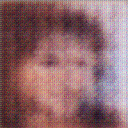
\includegraphics[width=150px]{500_fake_images/samples_5_293.png}%
\caption{A Close Up Of A Person Holding A Cell Phone}%
\end{figure}

%
\end{document}